% Editable slide deck entrypoint.
% Refresh generated facts first with: python -m src.cli analyse --no-compile

\PassOptionsToPackage{table}{xcolor}
\documentclass[aspectratio=169,12pt]{beamer}

\usetheme{metropolis}
\metroset{progressbar=frametitle, sectionpage=none, numbering=fraction}

\usepackage[utf8]{inputenc}
\usepackage[T1]{fontenc}
\usepackage[english]{babel}
\usepackage{graphicx}
\usepackage{booktabs}
\usepackage{tabularx}
\usepackage{array}
\usepackage{xcolor}
\usepackage{lmodern}
\usepackage{microtype}
\usepackage{tikz}
\usepackage{appendixnumberbeamer}
\usetikzlibrary{arrows.meta,positioning}

\definecolor{navy}{RGB}{30,58,95}
\definecolor{careblue}{RGB}{37,99,235}
\definecolor{medigreen}{RGB}{22,163,74}
\definecolor{headerblue}{RGB}{213,232,240}
\definecolor{midgray}{RGB}{107,114,128}
\definecolor{lightgray}{RGB}{245,245,245}

\setbeamercolor{frametitle}{bg=navy, fg=white}
\setbeamercolor{progress bar}{fg=careblue}
\setbeamercolor{alerted text}{fg=careblue}
\setbeamercolor{title separator}{fg=careblue}
\setbeamercolor{normal text}{fg=navy!85!black}
\setbeamercolor{background canvas}{bg=white}

\graphicspath{{../output/figures/}}
% AUTO-GENERATED: document macros
% Refresh with python -m src.cli analyse --no-compile.
\newcommand{\MediFlowBuildDate}{2026-04-15}

\newcommand{\MediFlowBuildTimestamp}{2026-04-15T15:33+02:00}

\newcommand{\MediFlowAnalysisRunLabel}{15 Apr 2026, 15:33}

\newcommand{\MediFlowAutoTag}{[AUTO-GENERATED INTERPRETATION]}

\newcommand{\MediFlowContextPath}{\detokenize{../output/report_context.json}}

\newcommand{\MediFlowGeneratedDir}{\detokenize{../output/generated}}

\newcommand{\MediFlowCareFlowRawRows}{26,179}

\newcommand{\MediFlowMediTrackRawRows}{17,262}

\newcommand{\MediFlowCareFlowRegisteredCases}{26,179}

\newcommand{\MediFlowMediTrackRegisteredCases}{17,165}

\newcommand{\MediFlowCareFlowFinishedCases}{20,456}

\newcommand{\MediFlowMediTrackFinishedCases}{6,123}

\newcommand{\MediFlowCareFlowFinishedPct}{78.1\%}

\newcommand{\MediFlowMediTrackFinishedPct}{35.7\%}

\newcommand{\MediFlowCareFlowOpenPct}{14.1\%}

\newcommand{\MediFlowMediTrackOpenPct}{56.8\%}

\newcommand{\MediFlowCareFlowCancelledPct}{7.7\%}

\newcommand{\MediFlowMediTrackCancelledPct}{7.6\%}

\newcommand{\MediFlowCareFlowMedianDays}{48 days}

\newcommand{\MediFlowMediTrackMedianDays}{57 days}

\newcommand{\MediFlowCareFlowMonthCoverage}{11/12 months}

\newcommand{\MediFlowMediTrackMonthCoverage}{12/12 months}

\newcommand{\MediFlowCareFlowLogicalOrderPct}{99.8\%}

\newcommand{\MediFlowMediTrackLogicalOrderPct}{82.3\%}

\newcommand{\MediFlowCareFlowInversionPct}{0.156\%}

\newcommand{\MediFlowMediTrackInversionPct}{46.0\%}

\newcommand{\MediFlowMediTrackSlashPct}{50.1\%}

\newcommand{\MediFlowMediTrackDashPct}{49.9\%}

\newcommand{\MediFlowMediTrackExactDuplicateRows}{81}

\newcommand{\MediFlowMediTrackCaseRowsRemoved}{16}

\newcommand{\MediFlowCareFlowHovedstadenPct}{93.9\%}

\newcommand{\MediFlowCareFlowSjaellandPct}{5.0\%}

\newcommand{\MediFlowMediTrackHovedstadenPct}{3.5\%}

\newcommand{\MediFlowMediTrackSjaellandPct}{94.6\%}

\newcommand{\MediFlowFoundationPoints}{%
\begin{itemize}
  \item We tested candidate file encodings to find an import setup that preserved the raw values.
  \item We read date columns as text first to find the real source formats before parsing them.
  \item We measured the slash and dash populations to find how mixed the messy date fields were.
  \item We separated exact duplicate rows from duplicate case IDs to find the true case grain.
  \item We marked risky metrics as exploratory to find which comparisons were safe to treat as headline results.
  \item We generated report facts from the script to keep the written outputs aligned with the current run.
\end{itemize}
}

\newcommand{\MediFlowCurrentRunHighlights}{%
\begin{itemize}
  \item CareFlow finished case rate (Completed): 78.1\%
  \item CareFlow open rate at year end: 14.1\%
  \item CareFlow median treatment time: 48 days
  \item MediTrack finished case rate (Done): 35.7\%
  \item MediTrack finish-before-registration rate: 46.0\%
  \item MediTrack RegisteredAt date styles: 50.1\% slash / 49.9\% dash
  \item MediTrack duplicate cleanup in the pipeline: 81 exact rows removed and 16 extra case rows collapsed
\end{itemize}
}

\newcommand{\MediFlowKpiRows}{%
Registered cases (2022) & 26,179 & 17,165 & Case-level comparison \\
Finished cases & 20,456 & 6,123 & Completed vs Done \\
Finished case rate & 78.1\% & 35.7\% & Same concept \\
Open rate & 14.1\% & 56.8\% & MediTrack groups Open, Pending, and In Progress \\
Cancelled rate & 7.7\% & 7.6\% & Comparable \\
Median treatment time & 48 days & 57 days & MediTrack exploratory \\
Finish before registration & 0.156\% & 46.0\% & Date-order check \\
}

\newcommand{\MediFlowScorecardRows}{%
Date format & OK: single YYYYMMDD format & Caution: mixed slash/dash timestamps (50.1\% slash, 49.9\% dash) \\
Parse rate & OK: 100.0\% & OK: 100.0\% \\
Reg <= assign & OK: 99.8\% & Caution: 82.3\% \\
Finish before reg & OK: 0.156\% & Fail: 46.0\% \\
Treatment-time KPI & OK: median 48 d & Exploratory: median 57 d \\
Temporal coverage & Caution: 11/12 months & OK: 12/12 months \\
Duplicates & OK: no duplicate case rows & Fail: 81 exact rows and 16 extra case rows required collapse \\
}

\newcommand{\MediFlowCareFlowCategoryRows}{%
HOME\_MON & 22.9\% & 78.3\% & 7.5\% \\
SURG\_PRE & 19.9\% & 79.7\% & 6.2\% \\
ACUTE & 14.9\% & 75.5\% & 10.4\% \\
REHAB & 13.8\% & 76.8\% & 9.1\% \\
OUTP\_FUP & 10.7\% & 81.2\% & 4.6\% \\
SURG\_POST & 9.5\% & 73.3\% & 12.6\% \\
DIAG & 8.4\% & 82.5\% & 3.4\% \\
}

\newcommand{\MediFlowMediTrackCategoryRows}{%
Kort Sag & 28.0\% & 37.3\% & 6.0\% \\
Pakke A & 22.1\% & 34.8\% & 8.4\% \\
Pakke B & 17.5\% & 32.8\% & 10.4\% \\
Forlob Y & 12.8\% & 38.8\% & 4.5\% \\
Revurdering & 10.9\% & 30.6\% & 12.6\% \\
Forlob X & 8.7\% & 40.2\% & 3.0\% \\
}

\newcommand{\MediFlowCareFlowRegionRows}{%
Hovedstaden & 93.9\% \\
Sjaelland & 5.0\% \\
Other & 1.1\% \\
}

\newcommand{\MediFlowMediTrackRegionRows}{%
Hovedstaden & 3.5\% \\
Sjaelland & 94.6\% \\
Other & 1.9\% \\
}

\newcommand{\MediFlowAutoExecSummary}{%
CareFlow supports a more direct KPI read in this run: 78.1\% finished, 14.1\% still open, and almost no finish-before-registration cases (0.156\%). MediTrack is still useful for case counts and status mix, but 46.0\% of finished cases fall before registration, so the 57 days treatment-time figure should stay a rough check.
}

\newcommand{\MediFlowAutoQualitySummary}{%
The two datasets needed different cleanup steps before comparison. CareFlow uses one date style and does not need case-level deduplication. MediTrack needed two extra checks: parsing mixed RegisteredAt date styles (50.1\% slash / 49.9\% dash) and collapsing 81 exact duplicate rows plus 16 extra RefNo rows to case level. That makes the status and volume comparisons stronger than the treatment-time comparison.
}

\newcommand{\MediFlowAutoGeoSummary}{%
CareFlow mostly uses Hovedstaden postcodes (93.9\%) with a smaller Sjaelland share (5.0\%). MediTrack mostly uses Sjaelland postcodes (94.6\%) with some Hovedstaden spillover (3.5\%). The postcode pools are synthetic and were chosen for readable visual separation, not to describe real regional activity.
}


\newcolumntype{Y}{>{\centering\arraybackslash}X}
\newcolumntype{L}{>{\raggedright\arraybackslash}X}
\newcolumntype{R}{>{\raggedleft\arraybackslash}X}
\def\tabularxcolumn#1{m{#1}}

\newcommand{\reciconcalendar}{%

\begin{tikzpicture}[scale=0.8, every node/.style={transform shape}]
\draw[rounded corners=0.08cm, line width=1.2pt, color=careblue] (0,0) rectangle (1.5,1.55);
\fill[careblue!14] (0,1.12) rectangle (1.5,1.55);
\draw[line width=1pt, color=careblue] (0.32,1.55) -- (0.32,1.8);
\draw[line width=1pt, color=careblue] (1.18,1.55) -- (1.18,1.8);
\draw[line width=0.9pt, color=careblue!70!black] (0.28,0.82) -- (0.66,0.42) -- (1.22,0.98);
\end{tikzpicture}}

\newcommand{\reciconwindow}{%

\begin{tikzpicture}[scale=0.8, every node/.style={transform shape}]
\draw[rounded corners=0.08cm, line width=1.2pt, color=careblue] (0,0) rectangle (1.7,1.35);
\fill[careblue!12] (0,1.05) rectangle (1.7,1.35);
\draw[line width=0.9pt, color=careblue!70!black] (0.22,0.77) -- (1.48,0.77);
\draw[line width=0.9pt, color=careblue!70!black] (0.22,0.48) -- (1.1,0.48);
\fill[medigreen!65] (0.24,0.21) rectangle (1.46,0.38);
\end{tikzpicture}}

\newcommand{\reciconcasegrain}{%

\begin{tikzpicture}[scale=0.8, every node/.style={transform shape}]
\draw[rounded corners=0.05cm, line width=1.1pt, color=careblue] (0.16,0.12) rectangle (1.3,1.1);
\draw[rounded corners=0.05cm, line width=1.1pt, color=careblue!70] (0,0.28) rectangle (1.14,1.26);
\draw[line width=0.9pt, color=careblue!75!black] (1.12,0.22) circle (0.28);
\draw[line width=0.9pt, color=careblue!75!black] (1.3,0.04) -- (1.54,-0.2);
\fill[careblue!15] (0.24,0.8) rectangle (0.98,0.96);
\fill[careblue!15] (0.24,0.5) rectangle (0.86,0.66);
\end{tikzpicture}}

\newcommand{\recicondictionary}{%

\begin{tikzpicture}[scale=0.8, every node/.style={transform shape}]
\draw[rounded corners=0.05cm, line width=1.2pt, color=medigreen] (0,0) rectangle (1.5,1.6);
\draw[line width=1pt, color=medigreen] (0.28,0.08) -- (0.28,1.52);
\fill[medigreen!12] (0.35,1.18) rectangle (1.28,1.4);
\draw[line width=0.8pt, color=medigreen!70!black] (0.42,0.92) -- (1.24,0.92);
\draw[line width=0.8pt, color=medigreen!70!black] (0.42,0.68) -- (1.24,0.68);
\draw[line width=0.8pt, color=medigreen!70!black] (0.42,0.44) -- (0.98,0.44);
\end{tikzpicture}}

\newcommand{\reciconrobust}{%

\begin{tikzpicture}[scale=0.8, every node/.style={transform shape}]
\draw[rounded corners=0.05cm, line width=1.1pt, color=medigreen] (0,0) rectangle (0.78,1.45);
\draw[rounded corners=0.05cm, line width=1.1pt, color=careblue] (0.92,0) rectangle (1.7,1.45);
\fill[medigreen!14] (0,0.98) rectangle (0.78,1.45);
\fill[careblue!12] (0.92,0.98) rectangle (1.7,1.45);
\draw[line width=0.9pt, color=medigreen!70!black] (0.18,0.58) -- (0.34,0.4) -- (0.58,0.72);
\node[color=careblue!75!black] at (1.31,0.56) {\Large ?};
\end{tikzpicture}}

\newcommand{\reciconpipeline}{%
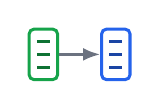
\begin{tikzpicture}[scale=0.8, every node/.style={transform shape}]
\draw[rounded corners=0.06cm, line width=1.1pt, color=medigreen] (0,0.25) rectangle (0.45,1.05);
\draw[rounded corners=0.06cm, line width=1.1pt, color=careblue] (1.15,0.25) rectangle (1.6,1.05);
\draw[-{Latex[length=2.2mm]}, line width=1.1pt, color=midgray] (0.47,0.65) -- (1.13,0.65);
\draw[line width=1pt, color=medigreen!70!black] (0.12,0.86) -- (0.33,0.86);
\draw[line width=1pt, color=medigreen!70!black] (0.12,0.65) -- (0.33,0.65);
\draw[line width=1pt, color=medigreen!70!black] (0.12,0.44) -- (0.33,0.44);
\draw[line width=1pt, color=careblue!70!black] (1.27,0.86) -- (1.48,0.86);
\draw[line width=1pt, color=careblue!70!black] (1.27,0.65) -- (1.48,0.65);
\draw[line width=1pt, color=careblue!70!black] (1.27,0.44) -- (1.48,0.44);
\end{tikzpicture}}

\title{MediFlow}
\subtitle{Synthetic comparison of CareFlow North and MediTrack East}
\author{Data quality, KPI logic, and repeatable reporting}
\date{Analysis run: \MediFlowAnalysisRunLabel}

\begin{document}

\maketitle

\begin{frame}{Data basis}
\renewcommand{\arraystretch}{1.22}
\arrayrulecolor{midgray}
\begin{tabularx}{\textwidth}{|L|Y|Y|}
\hline
\rowcolor{headerblue}
 & \textbf{\color{careblue}CareFlow North} & \textbf{\color{medigreen}MediTrack East} \\
\hline
Raw rows & \MediFlowCareFlowRawRows & \MediFlowMediTrackRawRows \\
\hline
\rowcolor{lightgray}
Rows in the 2022 window & \MediFlowCareFlowRegisteredCases & \MediFlowMediTrackRegisteredCases \\
\hline
Date style & One stable \texttt{YYYYMMDD} format & Mixed slash and dash timestamps \\
\hline
\rowcolor{lightgray}
Month coverage & \MediFlowCareFlowMonthCoverage & \MediFlowMediTrackMonthCoverage \\
\hline
Main read & Cleaner KPI source & Richer category source \\
\hline
\end{tabularx}

\vspace{0.35em}
{\small\color{midgray}Synthetic data, real workflow pattern: one easier source and one messier source.}
\end{frame}

\begin{frame}{Field mapping: what can compare?}
\renewcommand{\arraystretch}{1.18}
\arrayrulecolor{midgray}
\begin{tabularx}{\textwidth}{|L|L|L|}
\hline
\rowcolor{headerblue}
\textbf{Shared idea} & \textbf{\color{careblue}CareFlow} & \textbf{\color{medigreen}MediTrack} \\
\hline
Case reference & \texttt{CARE\_REF} & \texttt{RefNo} \\
\hline
\rowcolor{lightgray}
Registration date & \texttt{DT\_REG} & \texttt{RegisteredAt} \\
\hline
Assignment date & \texttt{DT\_ALLOC} & \texttt{AssignedOn} \\
\hline
\rowcolor{lightgray}
Cancelled date & \texttt{DT\_ABORT} & \texttt{CancelledOn} \\
\hline
Pathway start & \texttt{DT\_OPEN} & \texttt{StartPathway} \\
\hline
\rowcolor{lightgray}
Finished date idea & \texttt{max(DT\_END, DT\_CLOSE)} & \texttt{FinishedAt} \\
\hline
Category field & \texttt{TRACK} & \texttt{CareGroup} \\
\hline
\end{tabularx}

\vspace{0.35em}
{\small\color{midgray}The report compares shared concepts at case level. It does not join rows across systems.}
\end{frame}

\begin{frame}{Date fields: one common idea, two different systems}
\renewcommand{\arraystretch}{1.18}
\arrayrulecolor{midgray}
\begin{tabularx}{\textwidth}{|L|Y|Y|}
\hline
\rowcolor{headerblue}
\textbf{Check} & \textbf{\color{careblue}CareFlow North} & \textbf{\color{medigreen}MediTrack East} \\
\hline
Registration basis & \texttt{DT\_REG} & \texttt{RegisteredAt} \\
\hline
\rowcolor{lightgray}
Order check & \texttt{DT\_REG <= DT\_ALLOC} & \texttt{RegisteredAt <= AssignedOn} \\
\hline
Finished-date use & Safe headline KPI basis & Exploratory only \\
\hline
\rowcolor{lightgray}
Finish-before-registration & \MediFlowCareFlowInversionPct & \MediFlowMediTrackInversionPct \\
\hline
\end{tabularx}

\vspace{0.45em}
{\small\color{midgray}This is the core reason the two systems can share one deck while still needing different warnings.}
\end{frame}

\begin{frame}{Date cleaning: CareFlow Excel formula}
\small
The original exploration included helping users turn raw exports into usable Excel dates before any KPI work could start.

\vspace{0.7em}
Raw pattern: {\ttfamily YYYYMMDD} with \texttt{0} used as missing.

\vspace{0.8em}
\textbf{Excel formula}

\vspace{0.25em}
\colorbox{lightgray}{\parbox{\dimexpr\textwidth-2em\relax}{\small\ttfamily
=IF(A2=0,"",DATE(LEFT(TEXT(A2,"00000000"),4), MID(TEXT(A2,"00000000"),5,2), RIGHT(TEXT(A2,"00000000"),2)))}}

\vspace{0.8em}
{\scriptsize\color{midgray}The final report does not depend on Excel. The formula stays here because it explains the original exploration and the rule later encoded in Python.}
\end{frame}

\begin{frame}{Date cleaning: MediTrack Excel formula}
\small
The messy system needed a branch in the parsing logic because the same field mixes slash and dash timestamps.

\vspace{0.3em}
{\scriptsize\color{midgray}Current mix in \texttt{RegisteredAt}: \MediFlowMediTrackSlashPct\ slash / \MediFlowMediTrackDashPct\ dash}

\vspace{0.55em}
\textbf{Excel formula}

\vspace{0.15em}
\colorbox{lightgray}{\parbox{\dimexpr\textwidth-2em\relax}{\scriptsize\ttfamily
=IF(A2="","",IF(ISNUMBER(SEARCH("/",A2)),\\
\hspace*{1.5em}DATE(MID(A2,FIND("/",A2,FIND("/",A2)+1)+1,4),\\
\hspace*{3.0em}LEFT(A2,FIND("/",A2)-1),\\
\hspace*{3.0em}MID(A2,FIND("/",A2)+1,FIND("/",A2,FIND("/",A2)+1)-FIND("/",A2)-1)),\\
\hspace*{1.5em}DATE(RIGHT(LEFT(A2,10),4),MID(A2,4,2),LEFT(A2,2))))}}

\vspace{0.6em}
{\scriptsize\color{midgray}This logic is now mirrored in the Python parser, so the pipeline stays the source of truth.}
\end{frame}

\begin{frame}{Date fields: side-by-side data quality}
\vspace{0.45em}
\scriptsize
\renewcommand{\arraystretch}{1.18}
\arrayrulecolor{midgray}
\begin{tabularx}{\textwidth}{|L|Y|Y|}
\hline
\rowcolor{headerblue}
\textbf{Check} & \textbf{\color{careblue}CareFlow North} & \textbf{\color{medigreen}MediTrack East} \\
\hline
Date format & OK: single \texttt{YYYYMMDD} format & Caution: mixed slash / dash timestamps \\
\hline
\rowcolor{lightgray}
Parse rate & OK: 100.0\% & OK: 100.0\% \\
\hline
Reg $\leq$ assign & OK: \MediFlowCareFlowLogicalOrderPct & Caution: \MediFlowMediTrackLogicalOrderPct \\
\hline
\rowcolor{lightgray}
Finish before reg & OK: \MediFlowCareFlowInversionPct & Fail: \MediFlowMediTrackInversionPct \\
\hline
Temporal coverage & Caution: \MediFlowCareFlowMonthCoverage & OK: \MediFlowMediTrackMonthCoverage \\
\hline
\rowcolor{lightgray}
Duplicates & OK: none at case level & Fail: \MediFlowMediTrackExactDuplicateRows\ exact rows + \MediFlowMediTrackCaseRowsRemoved\ extra case rows \\
\hline
\end{tabularx}
\vfill
\par\scriptsize\color{midgray}The full scorecard figure still exists in the appendix and report, but the deck now keeps this view readable.
\end{frame}

\begin{frame}[shrink=12]{KPI overview (2022)}
\vspace{0.65em}
\begin{columns}[c]
  \begin{column}{0.48\textwidth}
    \centering
    {\fontsize{26}{30}\selectfont\color{careblue}\textbf{\MediFlowCareFlowRegisteredCases}}\\[0.18em]
    {\small\color{midgray}registered cases --- CareFlow}\\
    {\scriptsize\color{midgray}\MediFlowCareFlowMonthCoverage}
  \end{column}
  \begin{column}{0.48\textwidth}
    \centering
    {\fontsize{26}{30}\selectfont\color{medigreen}\textbf{\MediFlowMediTrackRegisteredCases}}\\[0.18em]
    {\small\color{midgray}registered cases --- MediTrack}\\
    {\scriptsize\color{midgray}\MediFlowMediTrackMonthCoverage}
  \end{column}
\end{columns}

\vspace{0.7em}
\renewcommand{\arraystretch}{1.2}
\begin{tabularx}{\textwidth}{|L|Y|Y|}
\hline
\rowcolor{headerblue}
\textbf{KPI} & \textbf{\color{careblue}CareFlow} & \textbf{\color{medigreen}MediTrack} \\
\hline
Finished case rate & \MediFlowCareFlowFinishedPct & \MediFlowMediTrackFinishedPct \\
\hline
\rowcolor{lightgray}
Open rate & \MediFlowCareFlowOpenPct & \MediFlowMediTrackOpenPct \\
\hline
Cancelled rate & \MediFlowCareFlowCancelledPct & \MediFlowMediTrackCancelledPct \\
\hline
\rowcolor{lightgray}
Median treatment time & \MediFlowCareFlowMedianDays & \MediFlowMediTrackMedianDays \\
\hline
\end{tabularx}

\vfill
{\scriptsize\color{midgray}MediTrack treatment time stays exploratory because \MediFlowMediTrackInversionPct\ of finished cases still fall before registration.}
\end{frame}

\begin{frame}{CareFlow: status by month}
\centering
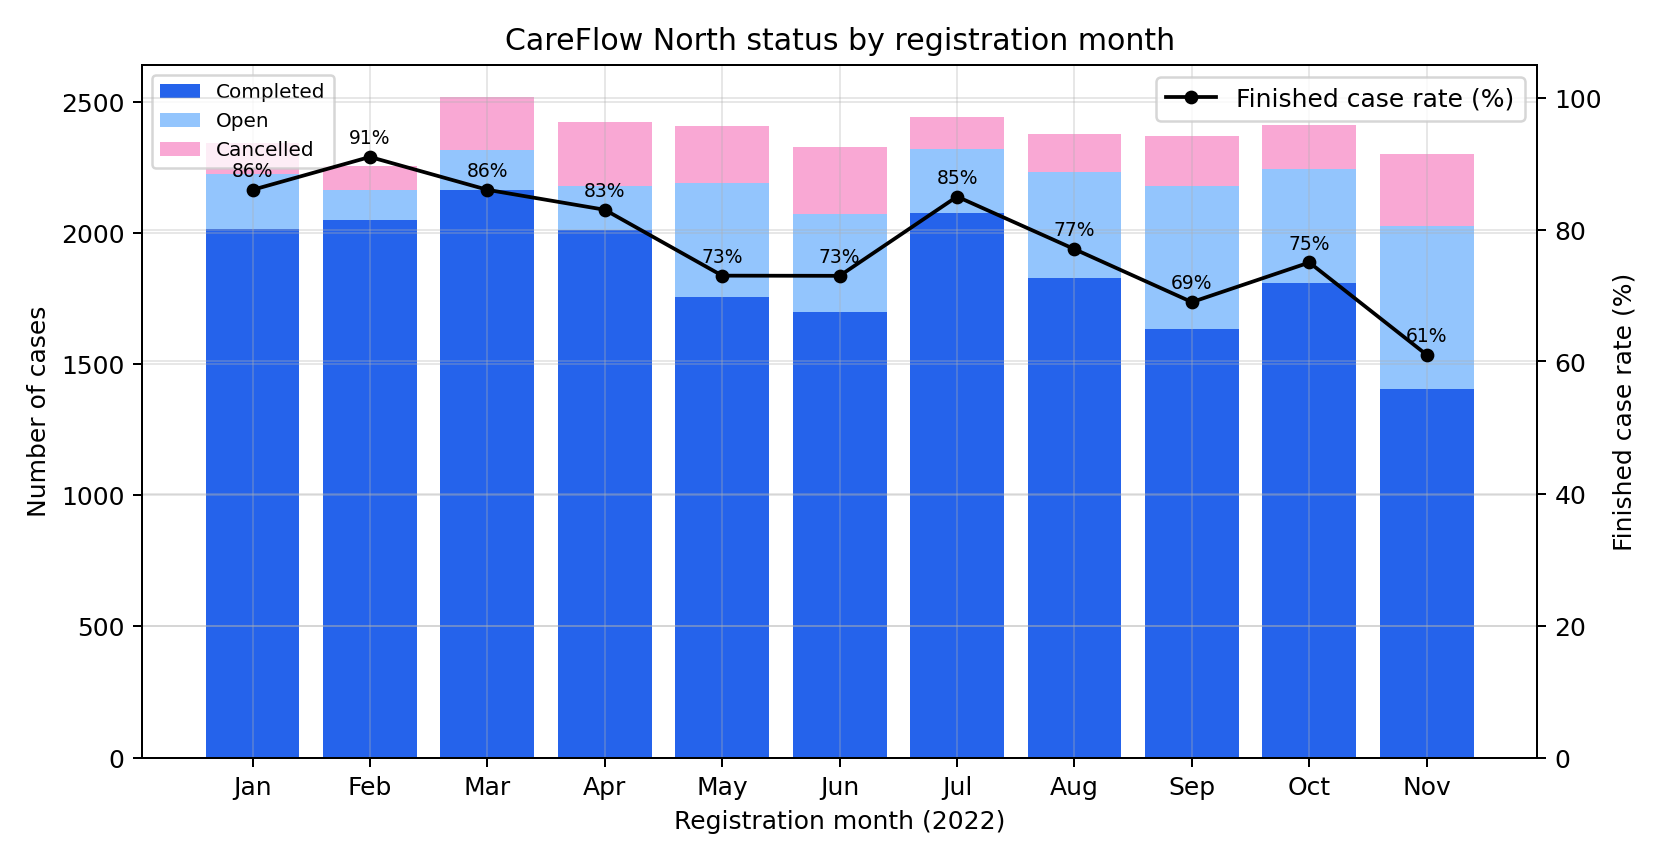
\includegraphics[width=\linewidth,height=0.82\textheight,keepaspectratio]{monthly_status_careflow.png}
\end{frame}

\begin{frame}{MediTrack: status by month}
\centering
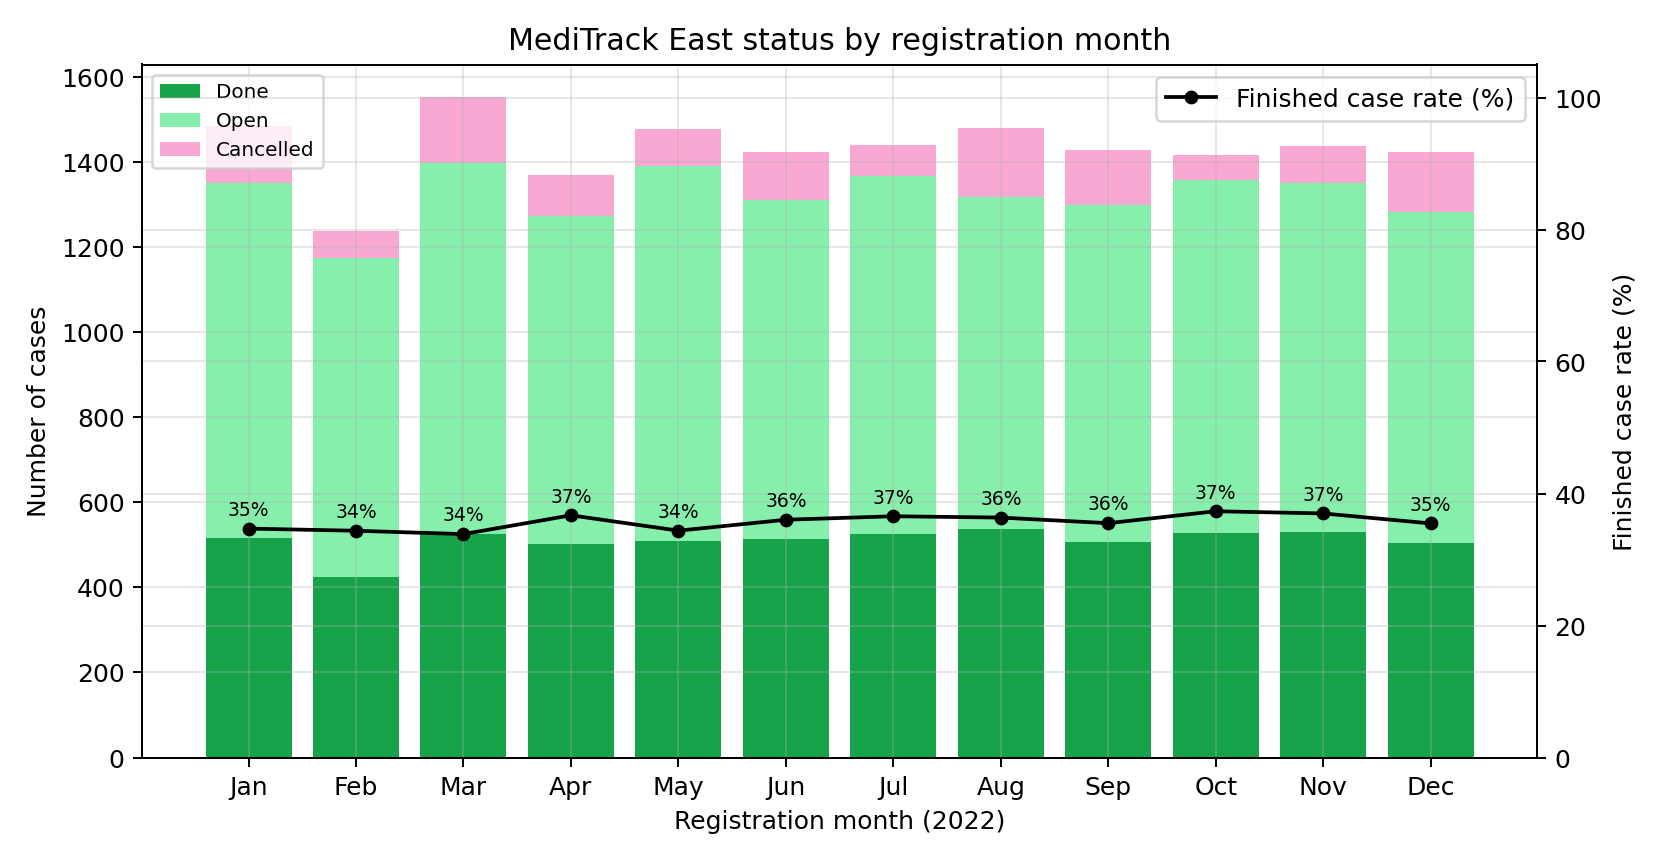
\includegraphics[width=\linewidth,height=0.82\textheight,keepaspectratio]{monthly_status_meditrack.png}
\end{frame}

\begin{frame}{Treatment time: finished cases}
\centering
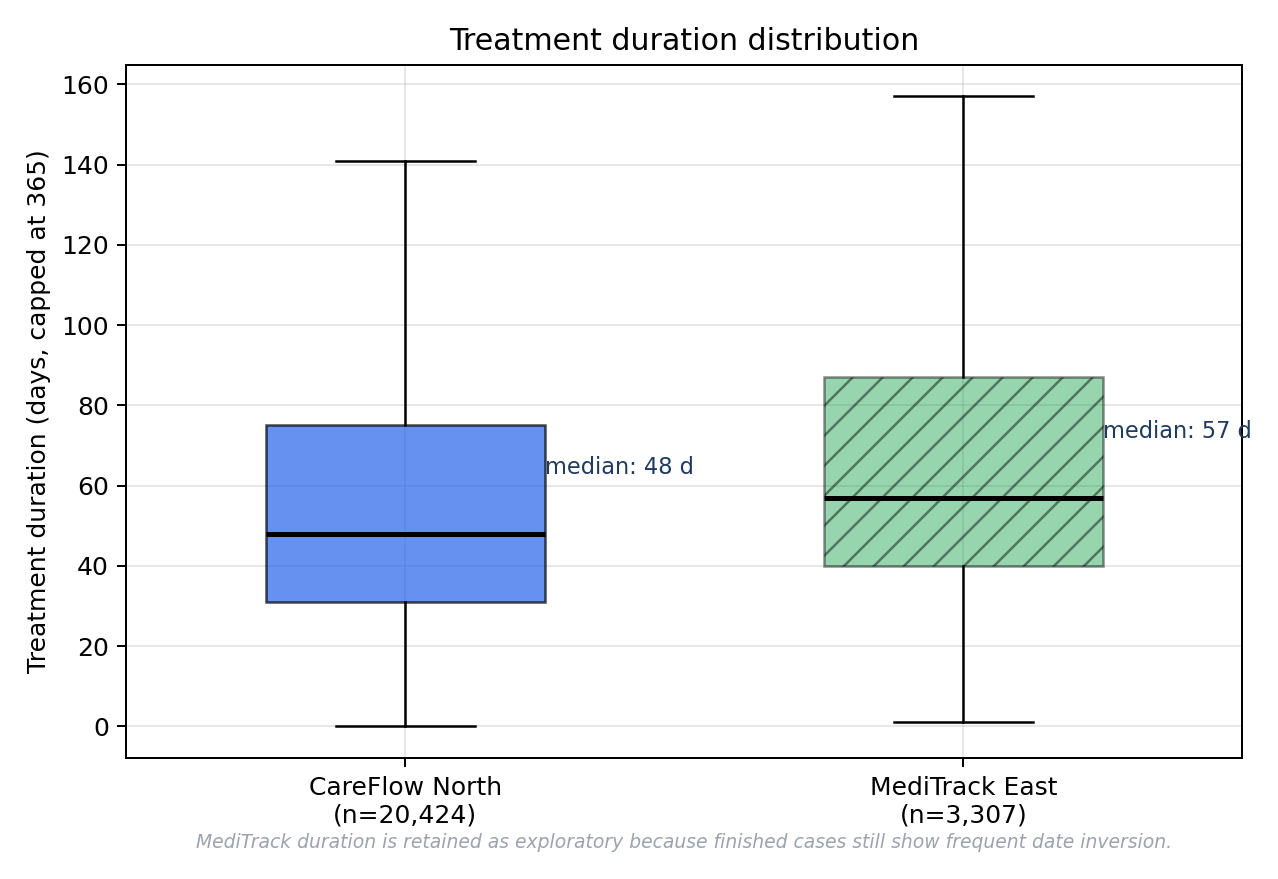
\includegraphics[width=\linewidth,height=0.82\textheight,keepaspectratio]{treatment_duration_boxplot.png}
\end{frame}

\begin{frame}{Automation pattern: MediTrack --- volume and variation}
\centering
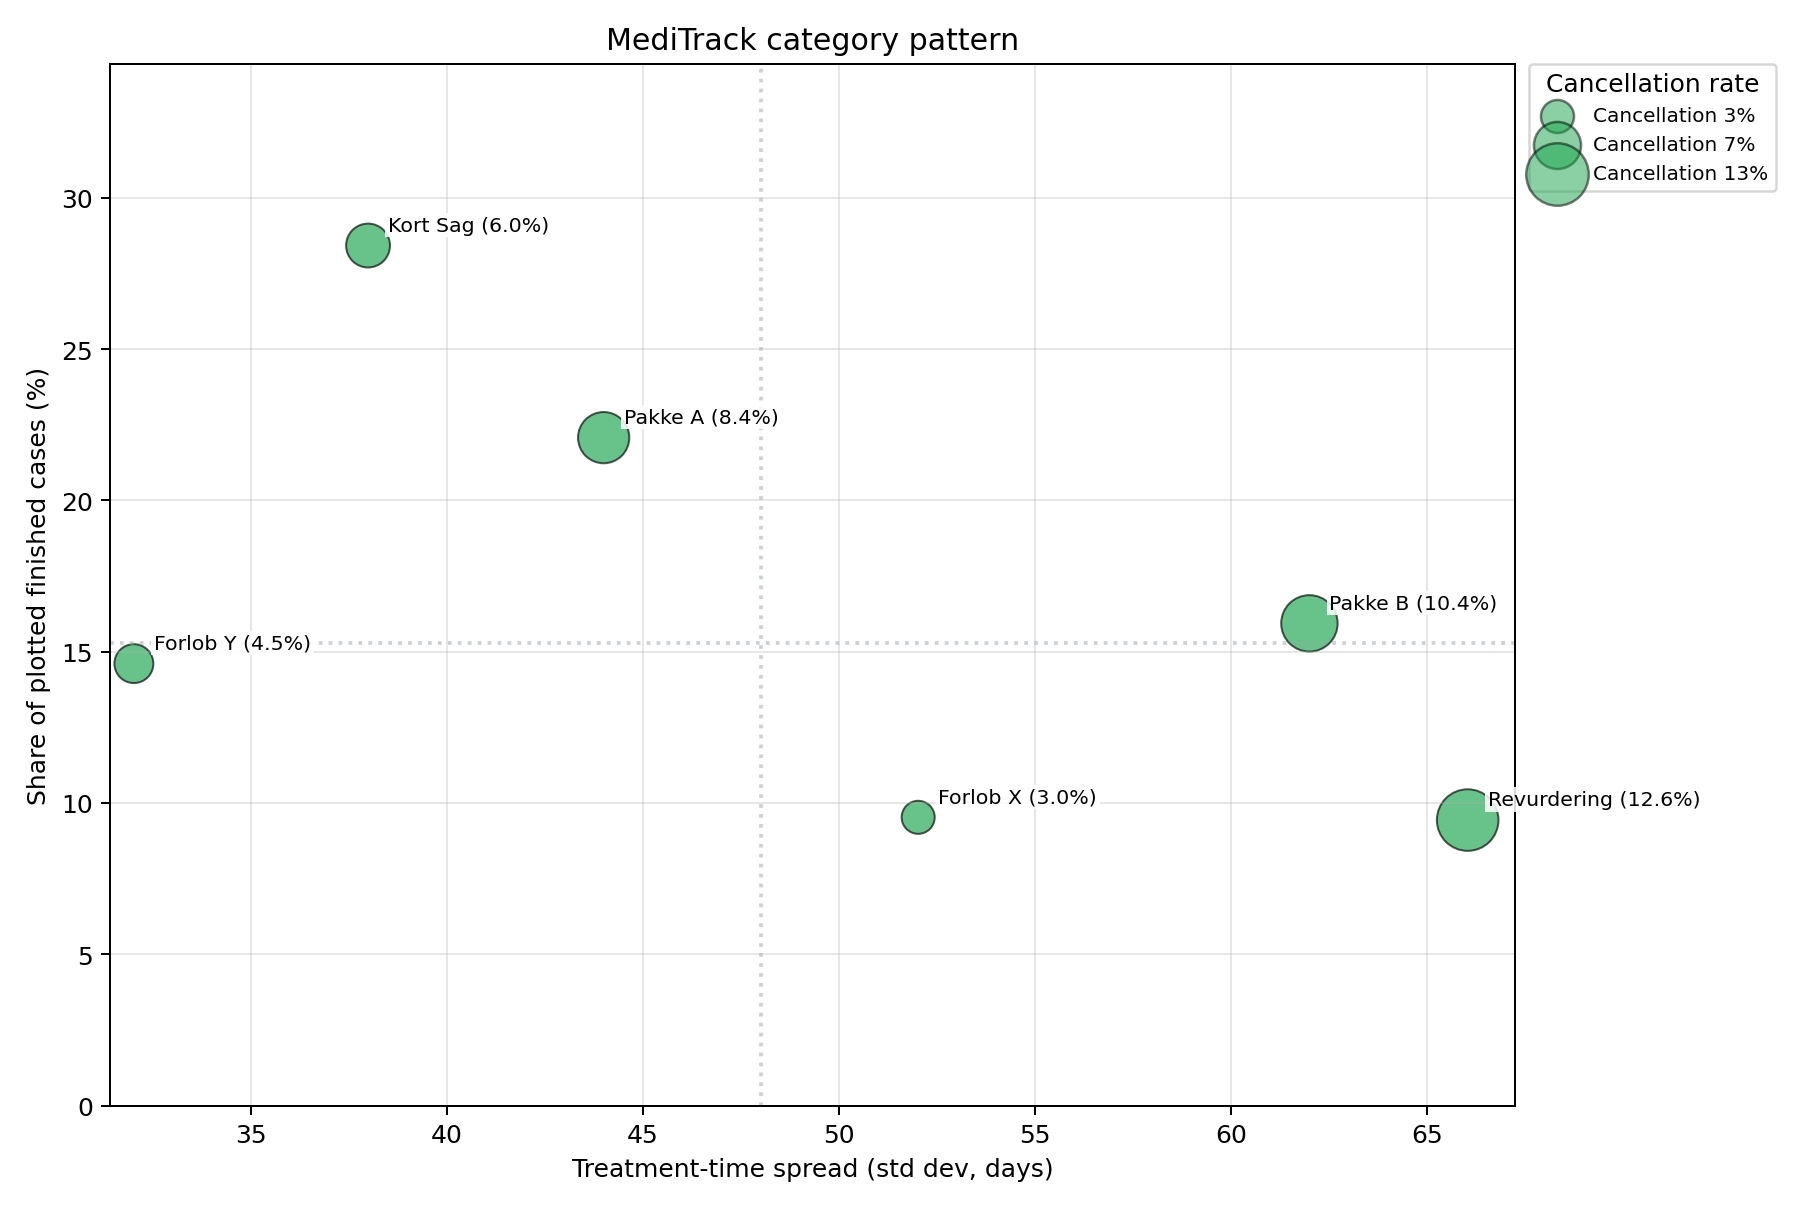
\includegraphics[width=\linewidth,height=0.82\textheight,keepaspectratio]{automation_matrix_meditrack.png}
\end{frame}

\begin{frame}{Recommendations: fix now}
\vspace{0.4em}
\begin{columns}[c]
  \begin{column}{0.32\textwidth}
    \centering
    \reciconcalendar\\[0.55em]
    \textbf{Standardise date exports}

    \small Use one clear date style in the messy system.
  \end{column}
  \begin{column}{0.32\textwidth}
    \centering
    \reciconwindow\\[0.55em]
    \textbf{Define complete reporting windows}

    \small Make month coverage explicit so the year view is not ambiguous.
  \end{column}
  \begin{column}{0.32\textwidth}
    \centering
    \reciconcasegrain\\[0.55em]
    \textbf{Keep case grain explicit}

    \small Make deduplication rules part of the handover, not hidden cleanup.
  \end{column}
\end{columns}
\end{frame}

\begin{frame}{Recommendations: build next}
\vspace{0.4em}
\begin{columns}[c]
  \begin{column}{0.32\textwidth}
    \centering
    \recicondictionary\\[0.55em]
    \textbf{Publish field definitions}

    \small A short data dictionary would remove a lot of uncertainty.
  \end{column}
  \begin{column}{0.32\textwidth}
    \centering
    \reciconrobust\\[0.55em]
    \textbf{Separate robust and exploratory KPIs}

    \small Keep the strong numbers visible without overstating the weaker ones.
  \end{column}
  \begin{column}{0.32\textwidth}
    \centering
    \reciconpipeline\\[0.55em]
    \textbf{Automate the intake checks}

    \small Parsing, deduplication, coverage checks, and report refresh belong in one workflow.
  \end{column}
\end{columns}
\end{frame}

\appendix

\begin{frame}{Appendix: date-field completeness}
\centering
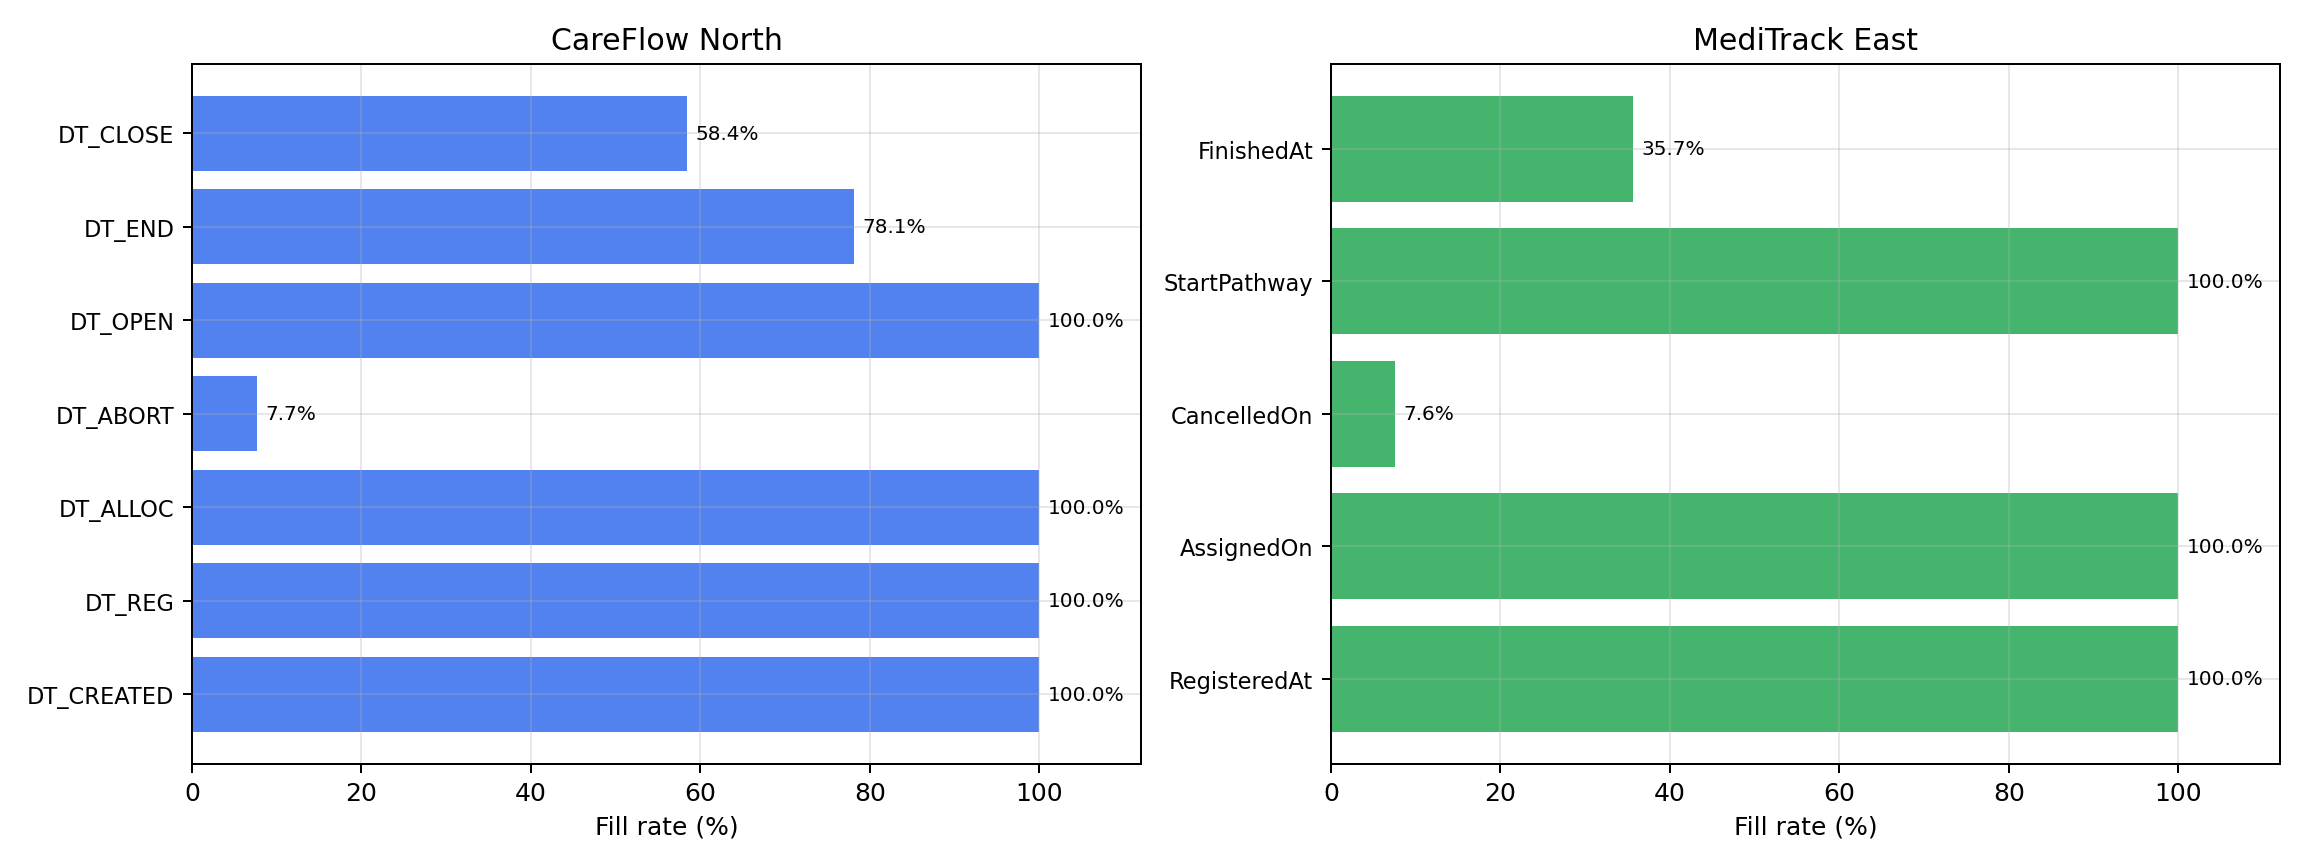
\includegraphics[width=\linewidth,height=0.82\textheight,keepaspectratio]{missing_date_fields.png}
\end{frame}

\begin{frame}{Appendix: date-field spans and outliers}
\centering
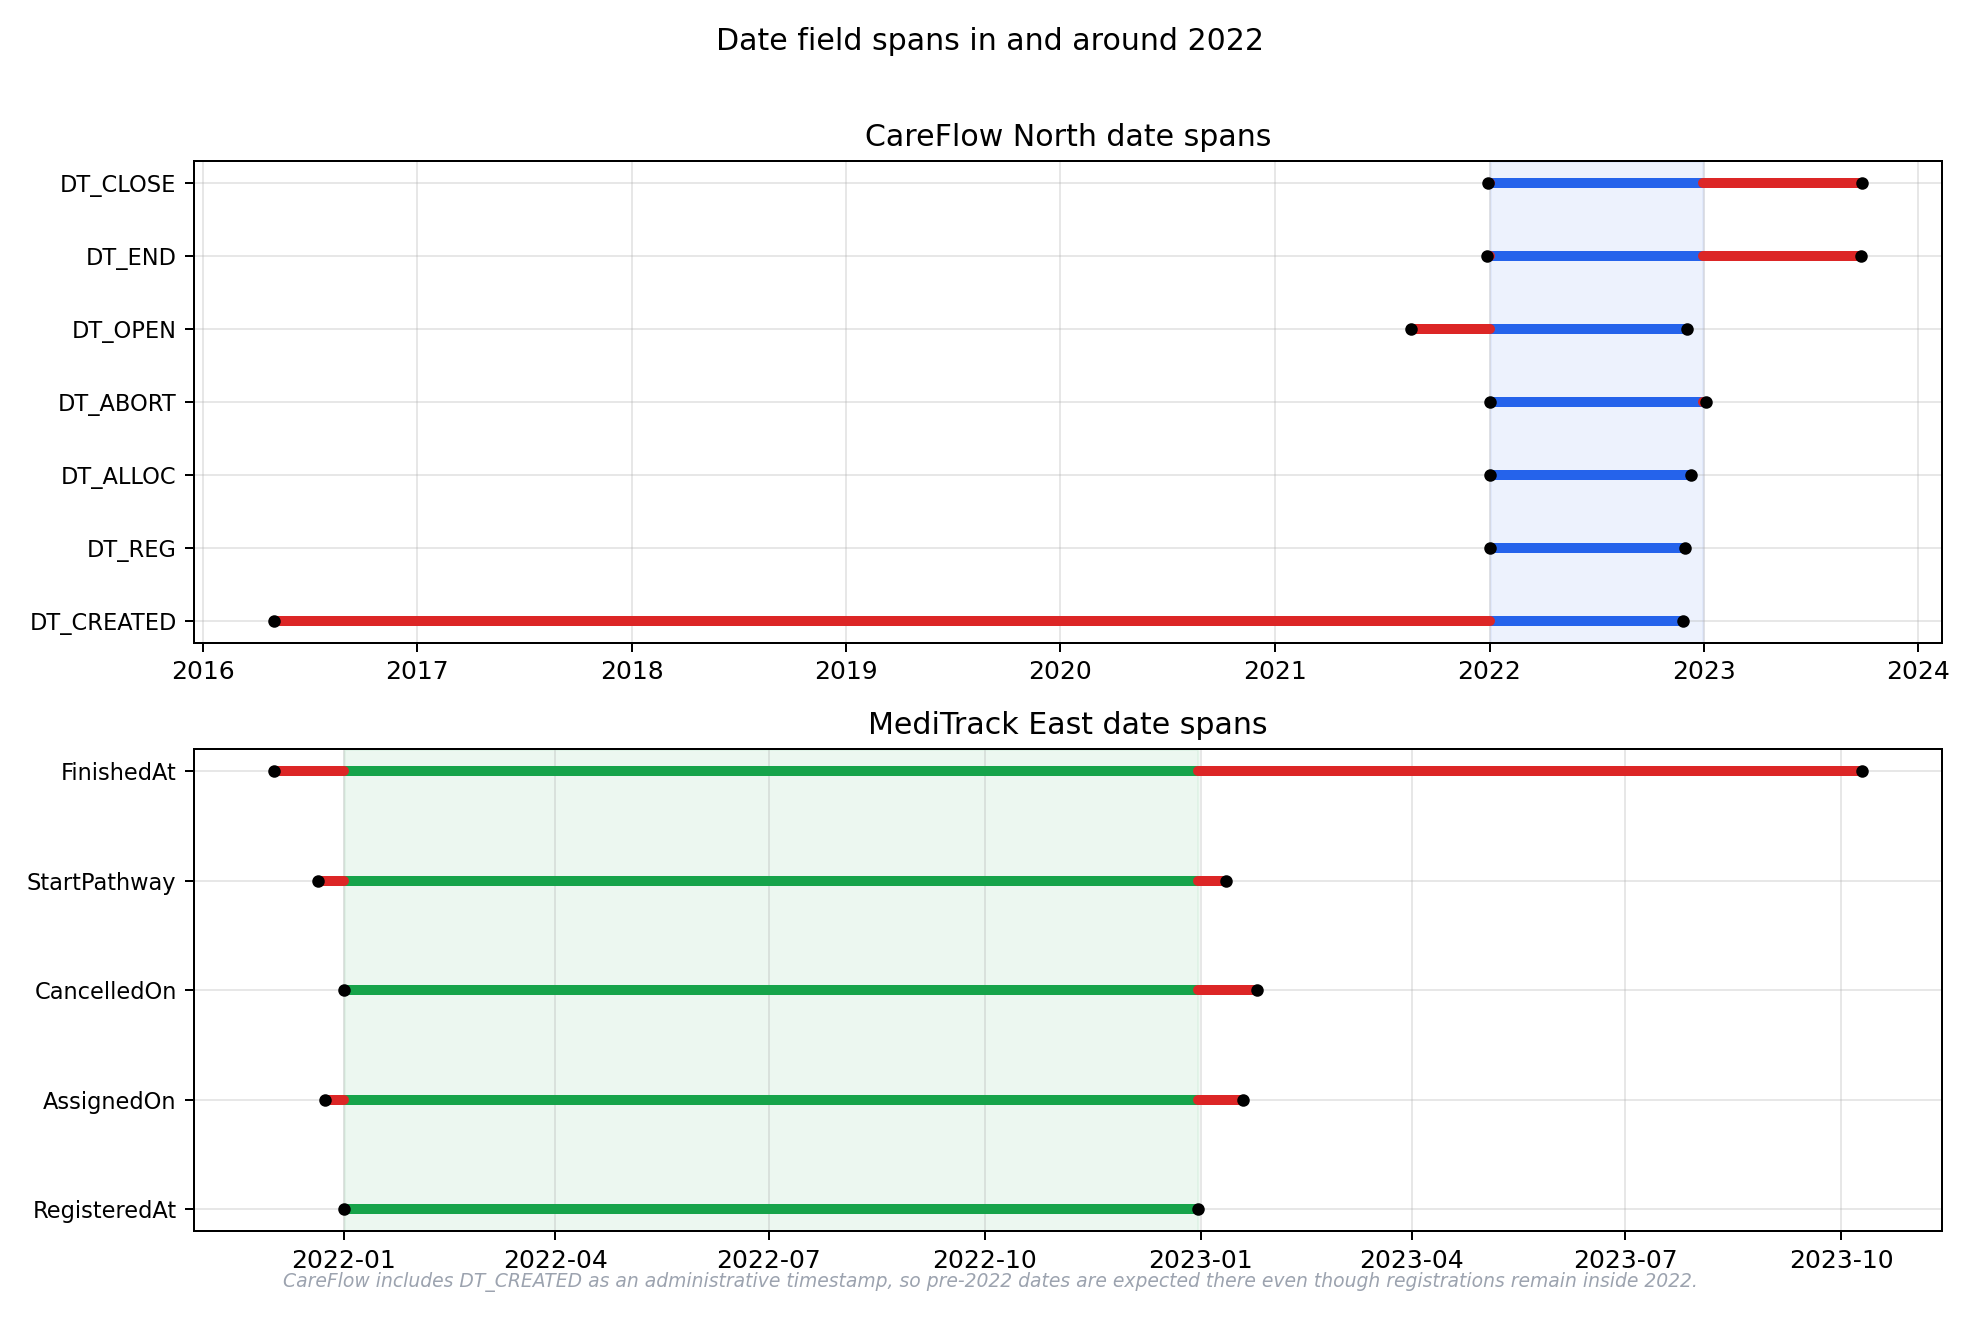
\includegraphics[width=\linewidth,height=0.82\textheight,keepaspectratio]{date_span_outliers.png}
\end{frame}

\begin{frame}{Appendix: KPI comparison}
\centering
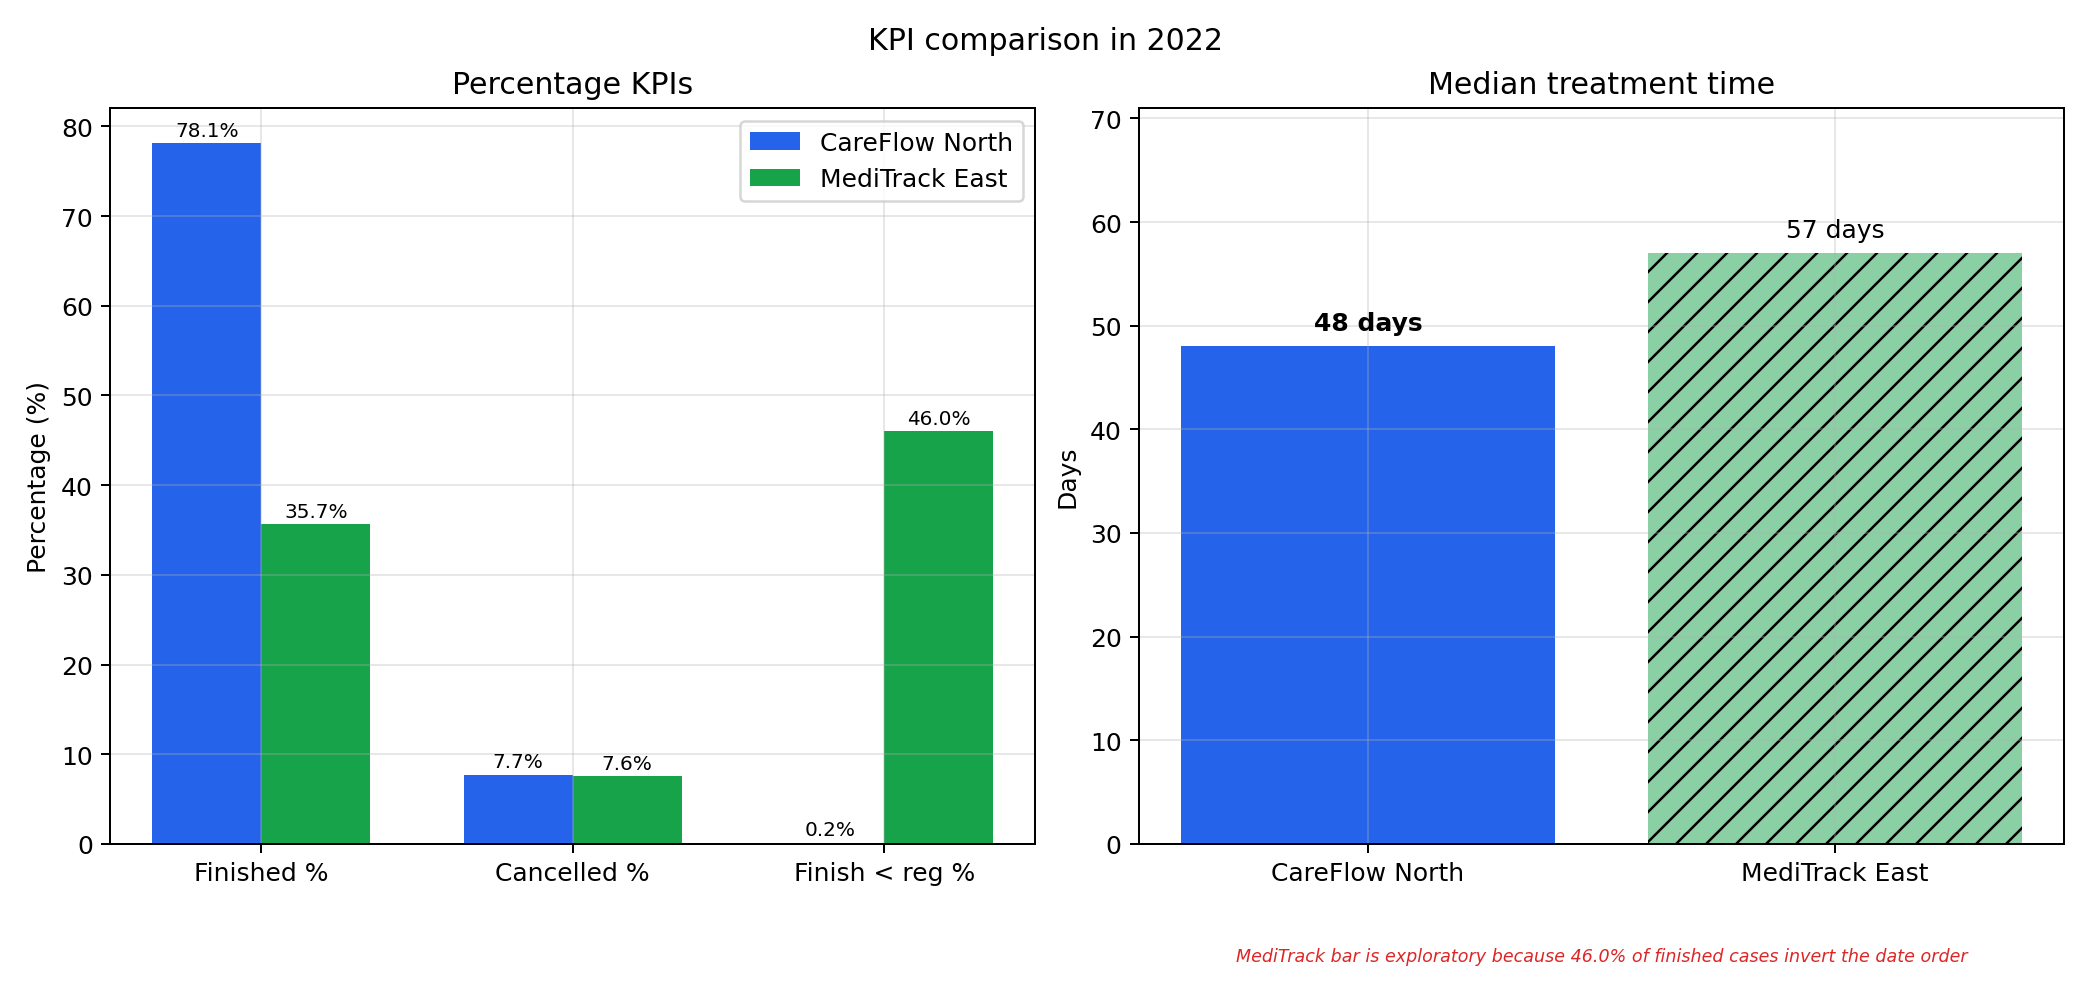
\includegraphics[width=\linewidth,height=0.82\textheight,keepaspectratio]{kpi_comparison.png}
\end{frame}

\begin{frame}{Appendix: monthly registration volume}
\centering
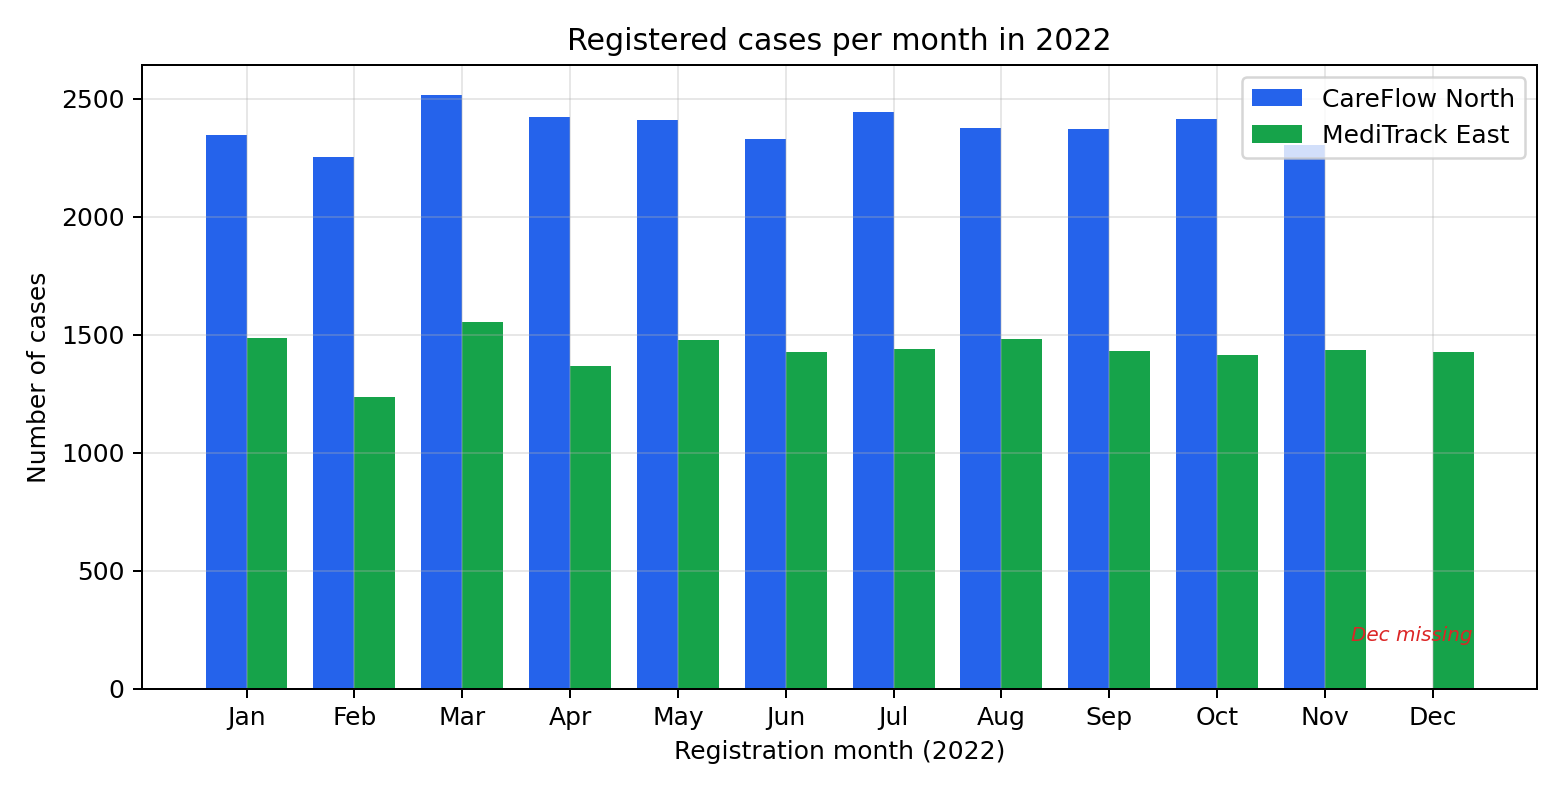
\includegraphics[width=\linewidth,height=0.82\textheight,keepaspectratio]{monthly_volume_2022.png}
\end{frame}

\begin{frame}{Appendix: synthetic postcode geography}
\centering
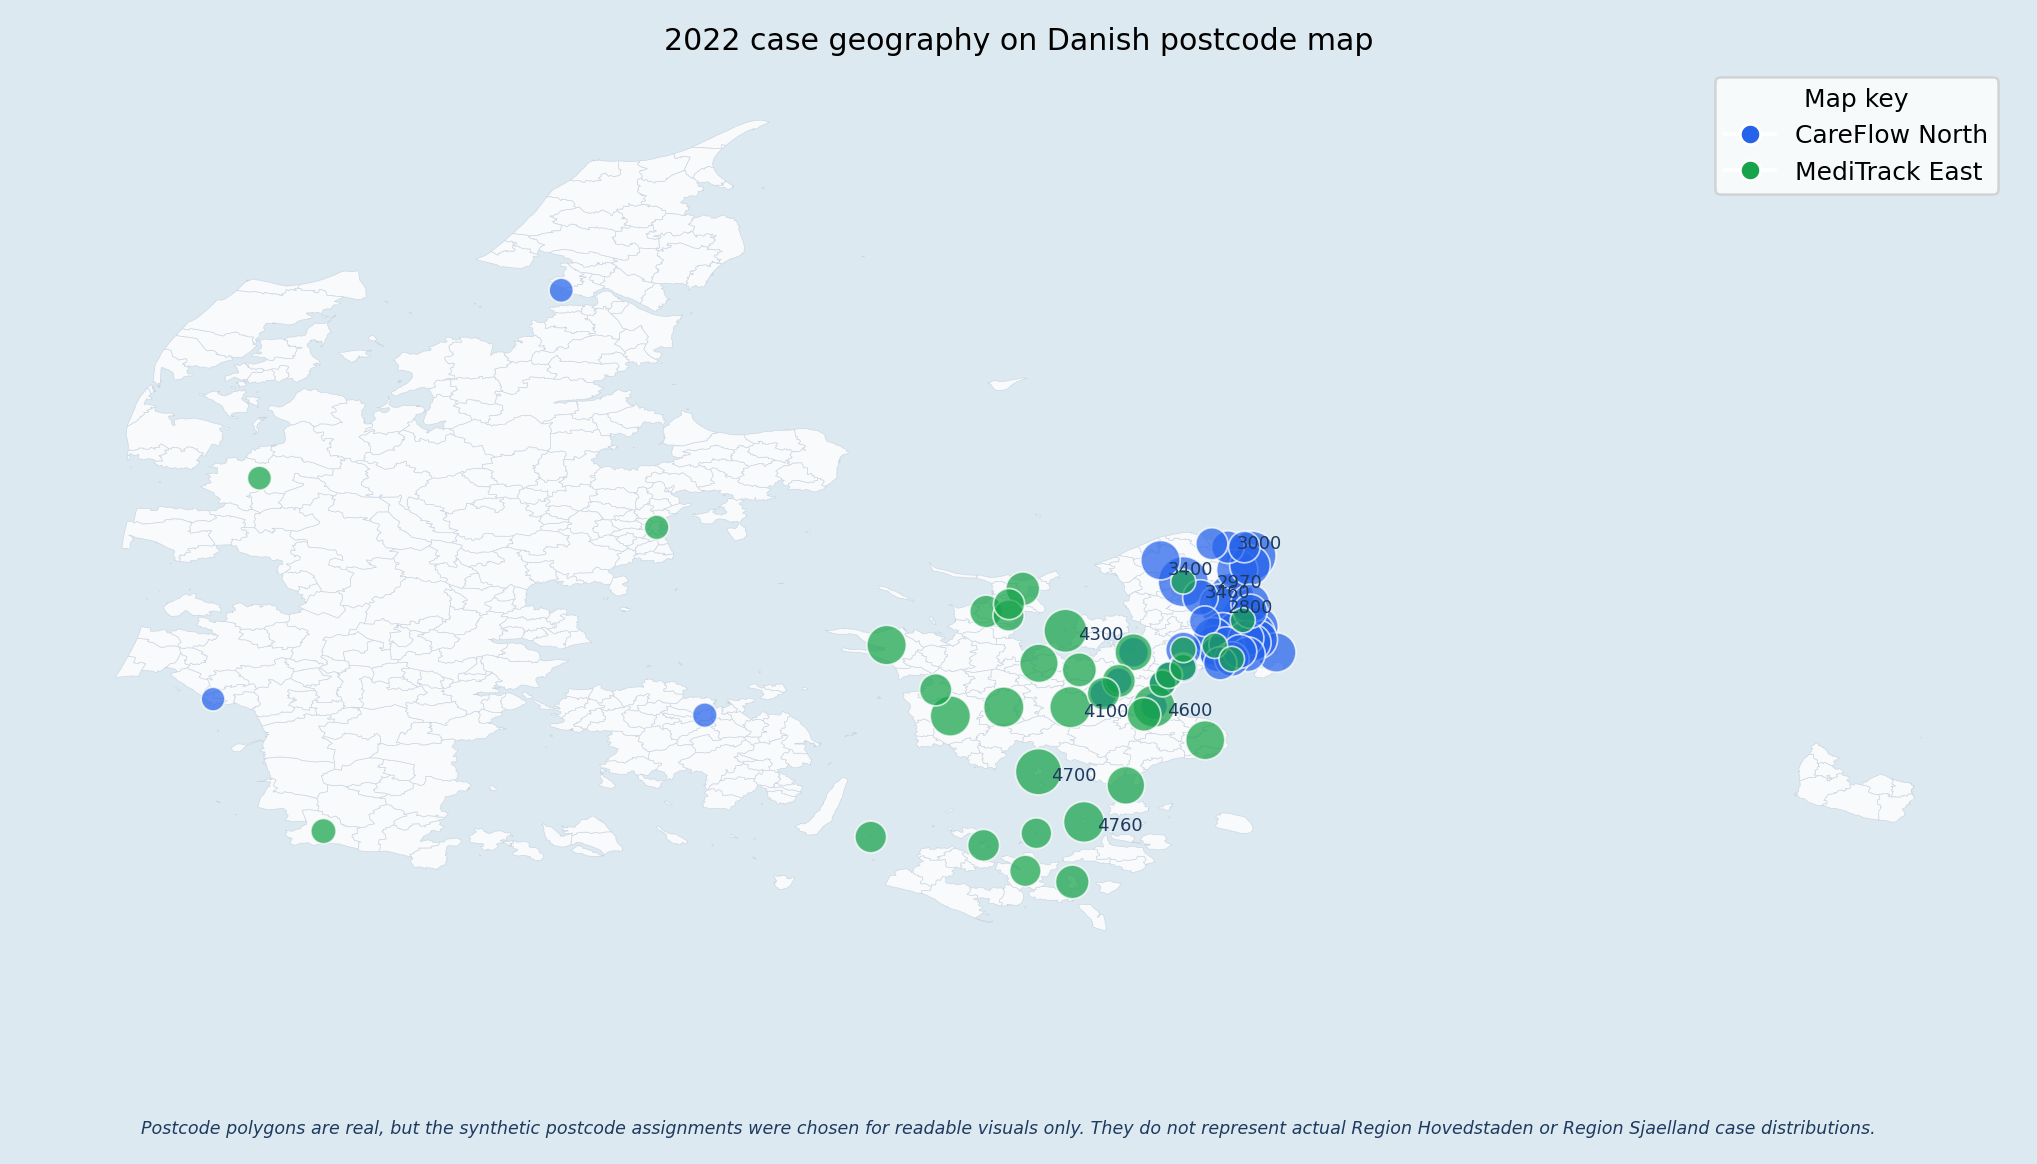
\includegraphics[width=\linewidth,height=0.82\textheight,keepaspectratio]{geo_top15_postalcodes.png}
\end{frame}

\begin{frame}{Appendix: CareFlow category pattern}
\centering
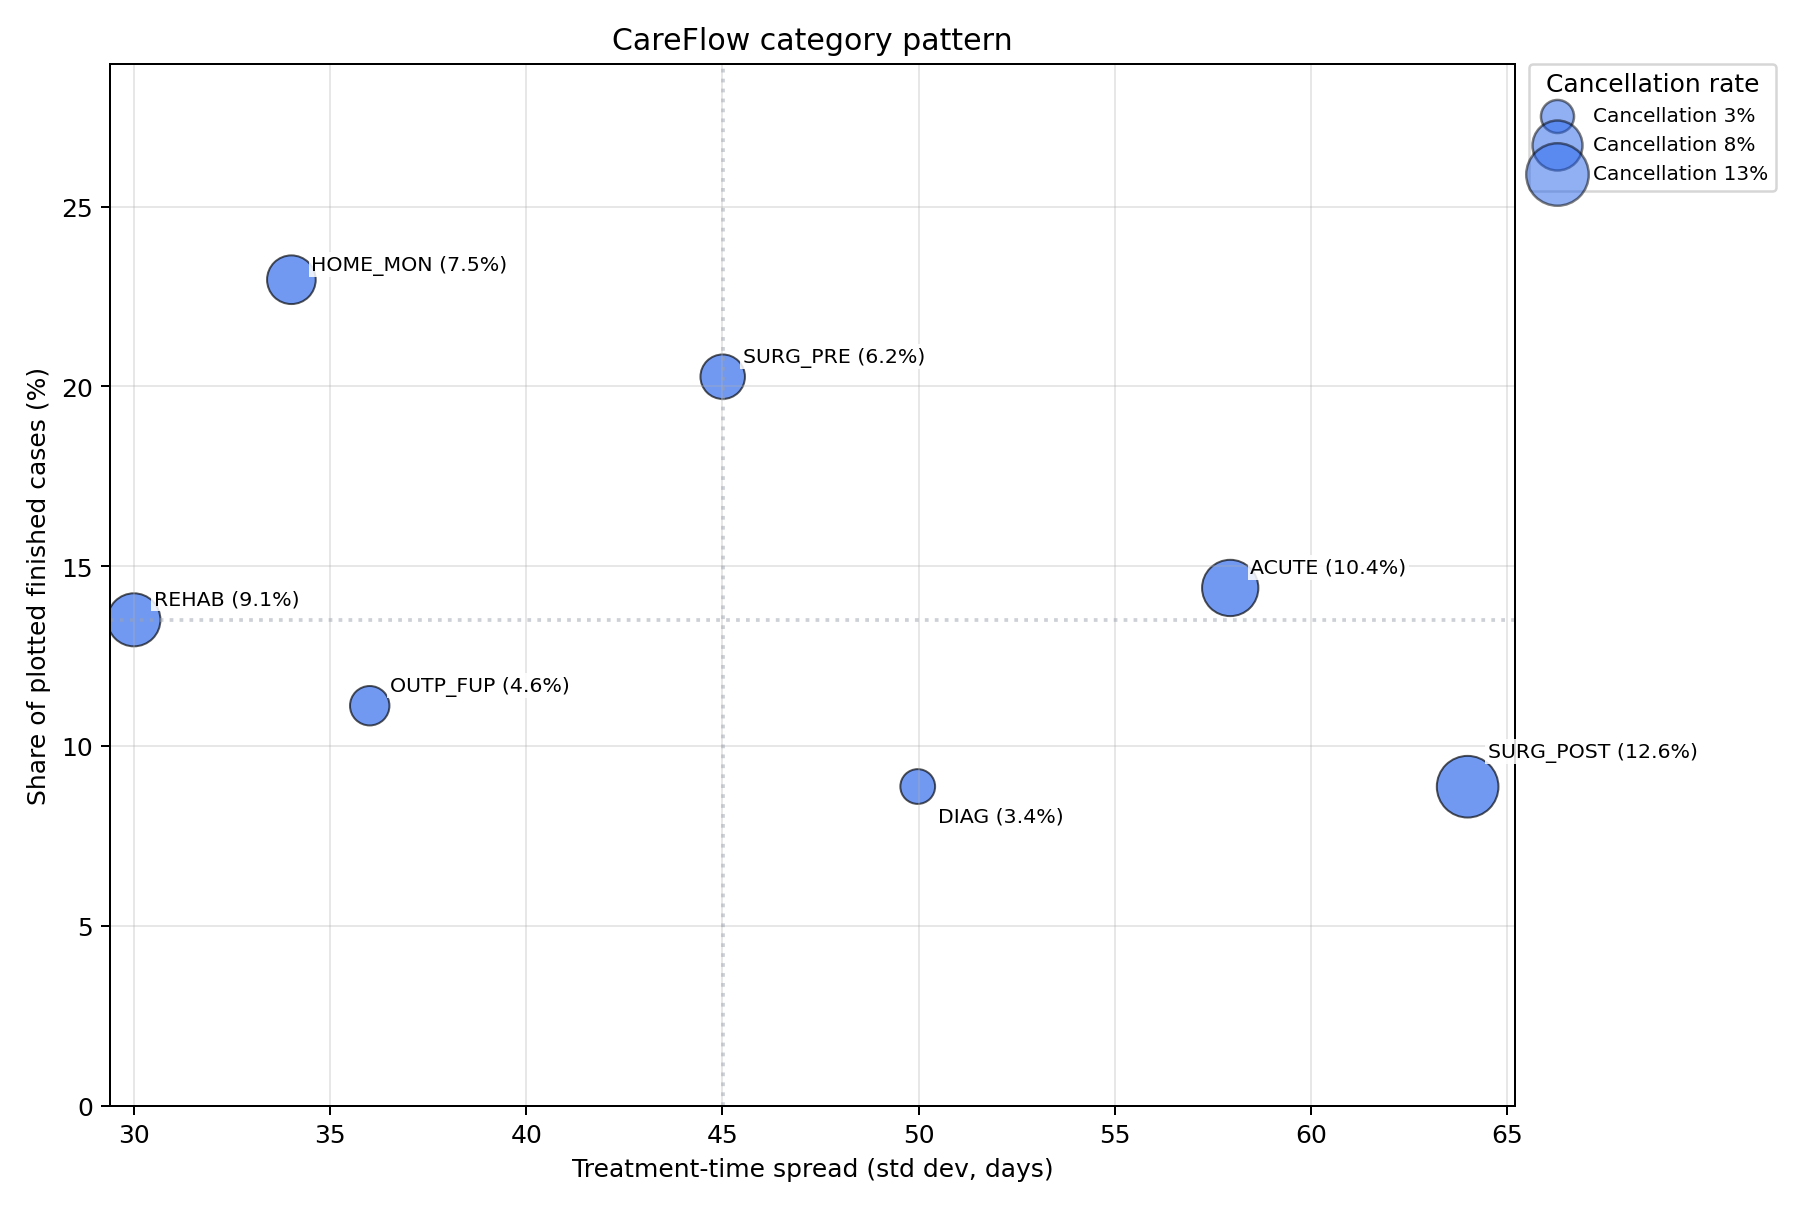
\includegraphics[width=\linewidth,height=0.82\textheight,keepaspectratio]{automation_matrix_careflow.png}
\end{frame}

\begin{frame}{Appendix: combined category pattern}
\centering
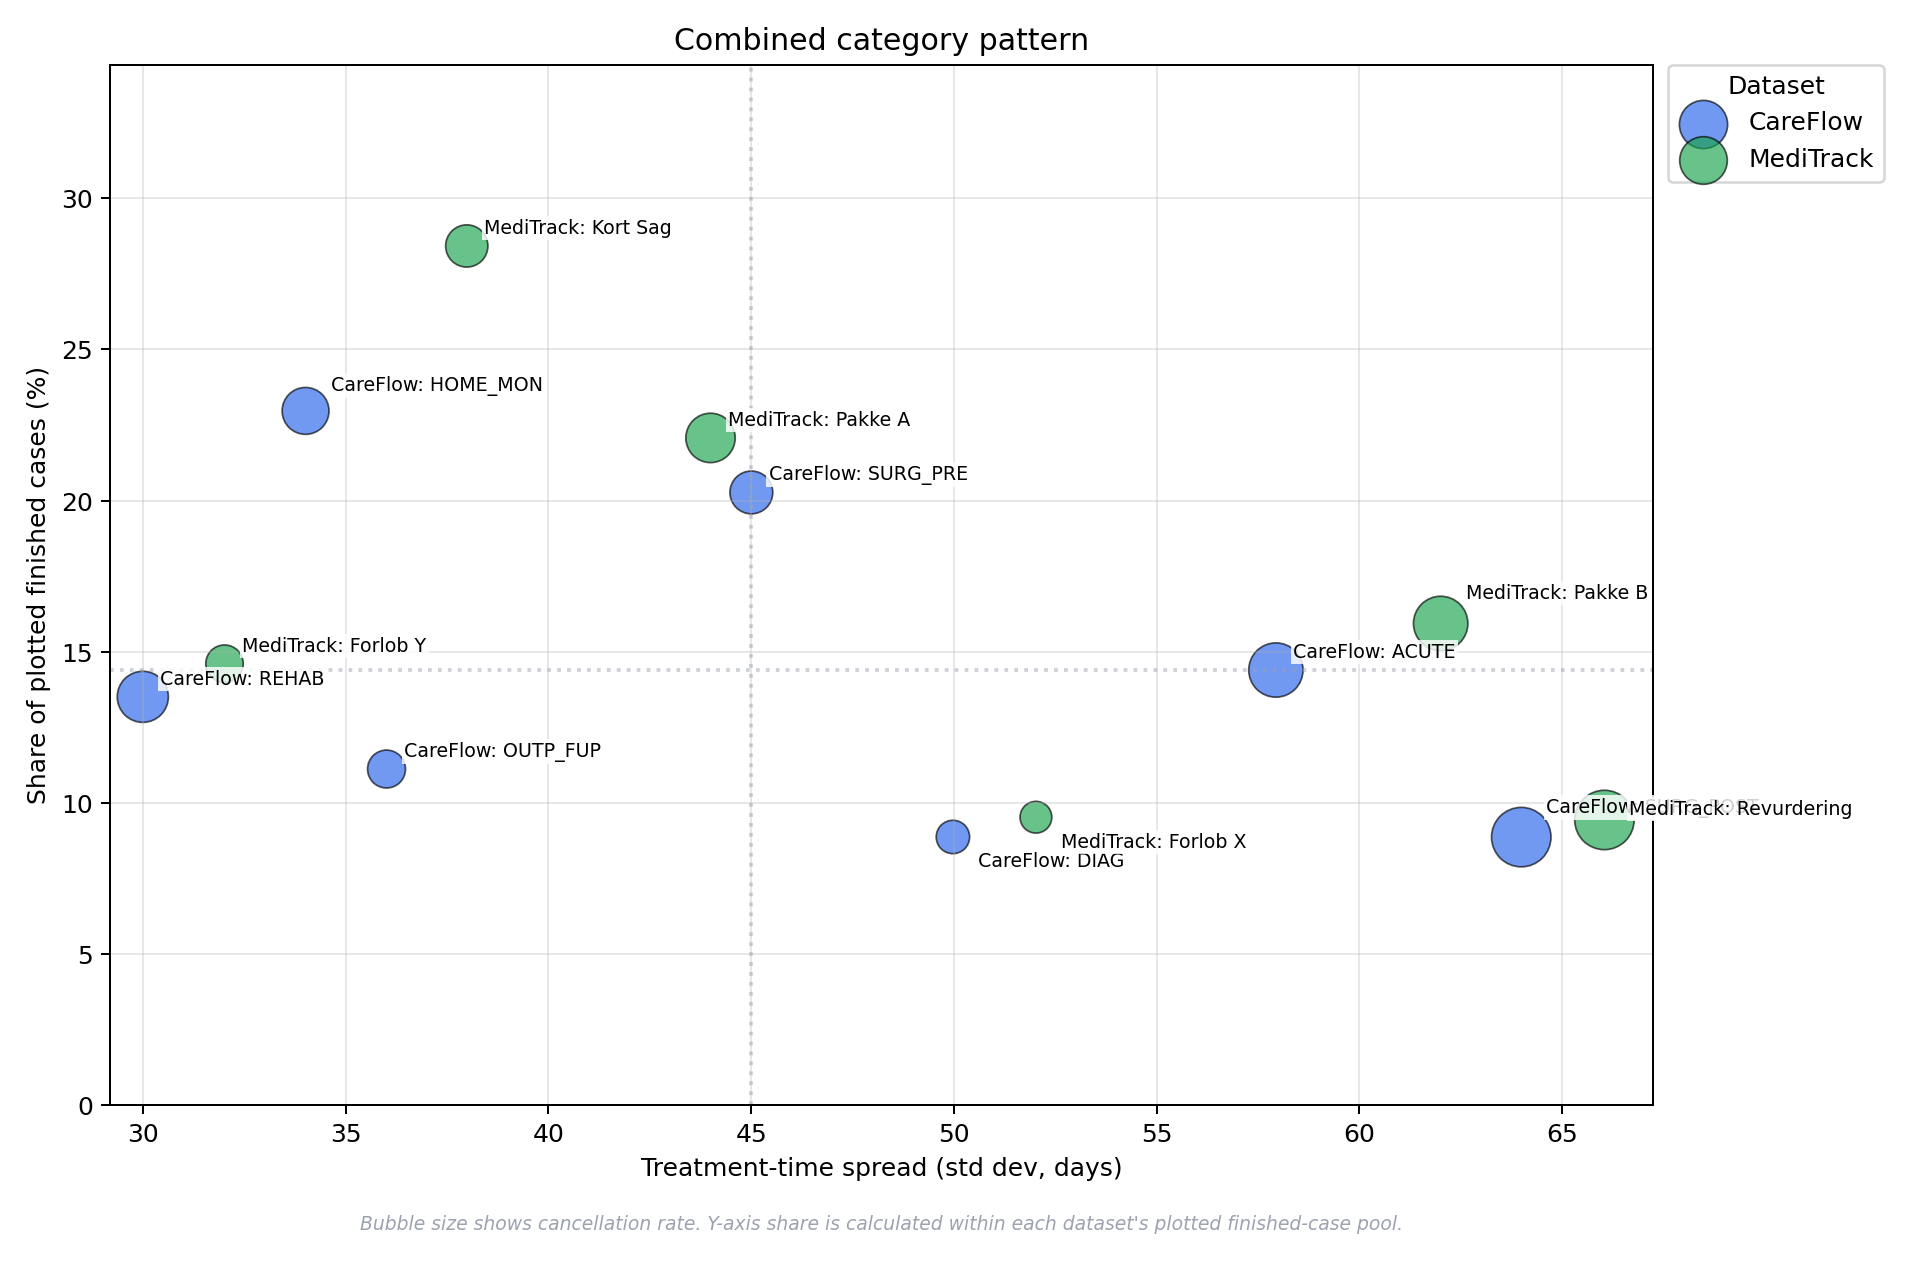
\includegraphics[width=\linewidth,height=0.82\textheight,keepaspectratio]{automation_matrix_combined.png}
\end{frame}

\end{document}
